% Options for packages loaded elsewhere
\PassOptionsToPackage{unicode}{hyperref}
\PassOptionsToPackage{hyphens}{url}
%
\documentclass[
  french,
]{article}
\usepackage{amsmath,amssymb}
\usepackage{lmodern}
\usepackage{ifxetex,ifluatex}
\ifnum 0\ifxetex 1\fi\ifluatex 1\fi=0 % if pdftex
  \usepackage[T1]{fontenc}
  \usepackage[utf8]{inputenc}
  \usepackage{textcomp} % provide euro and other symbols
\else % if luatex or xetex
  \usepackage{unicode-math}
  \defaultfontfeatures{Scale=MatchLowercase}
  \defaultfontfeatures[\rmfamily]{Ligatures=TeX,Scale=1}
\fi
% Use upquote if available, for straight quotes in verbatim environments
\IfFileExists{upquote.sty}{\usepackage{upquote}}{}
\IfFileExists{microtype.sty}{% use microtype if available
  \usepackage[]{microtype}
  \UseMicrotypeSet[protrusion]{basicmath} % disable protrusion for tt fonts
}{}
\makeatletter
\@ifundefined{KOMAClassName}{% if non-KOMA class
  \IfFileExists{parskip.sty}{%
    \usepackage{parskip}
  }{% else
    \setlength{\parindent}{0pt}
    \setlength{\parskip}{6pt plus 2pt minus 1pt}}
}{% if KOMA class
  \KOMAoptions{parskip=half}}
\makeatother
\usepackage{xcolor}
\IfFileExists{xurl.sty}{\usepackage{xurl}}{} % add URL line breaks if available
\IfFileExists{bookmark.sty}{\usepackage{bookmark}}{\usepackage{hyperref}}
\hypersetup{
  pdftitle={Synthèse des réponses au questionnaire d'évaluation du 3.3},
  pdfauthor={Nicolas Bressoud},
  pdflang={fr},
  hidelinks,
  pdfcreator={LaTeX via pandoc}}
\urlstyle{same} % disable monospaced font for URLs
\usepackage[margin=1in]{geometry}
\usepackage{longtable,booktabs,array}
\usepackage{calc} % for calculating minipage widths
% Correct order of tables after \paragraph or \subparagraph
\usepackage{etoolbox}
\makeatletter
\patchcmd\longtable{\par}{\if@noskipsec\mbox{}\fi\par}{}{}
\makeatother
% Allow footnotes in longtable head/foot
\IfFileExists{footnotehyper.sty}{\usepackage{footnotehyper}}{\usepackage{footnote}}
\makesavenoteenv{longtable}
\usepackage{graphicx}
\makeatletter
\def\maxwidth{\ifdim\Gin@nat@width>\linewidth\linewidth\else\Gin@nat@width\fi}
\def\maxheight{\ifdim\Gin@nat@height>\textheight\textheight\else\Gin@nat@height\fi}
\makeatother
% Scale images if necessary, so that they will not overflow the page
% margins by default, and it is still possible to overwrite the defaults
% using explicit options in \includegraphics[width, height, ...]{}
\setkeys{Gin}{width=\maxwidth,height=\maxheight,keepaspectratio}
% Set default figure placement to htbp
\makeatletter
\def\fps@figure{htbp}
\makeatother
\setlength{\emergencystretch}{3em} % prevent overfull lines
\providecommand{\tightlist}{%
  \setlength{\itemsep}{0pt}\setlength{\parskip}{0pt}}
\setcounter{secnumdepth}{5}
\ifxetex
  % Load polyglossia as late as possible: uses bidi with RTL langages (e.g. Hebrew, Arabic)
  \usepackage{polyglossia}
  \setmainlanguage[]{french}
\else
  \usepackage[main=french]{babel}
% get rid of language-specific shorthands (see #6817):
\let\LanguageShortHands\languageshorthands
\def\languageshorthands#1{}
\fi
\ifluatex
  \usepackage{selnolig}  % disable illegal ligatures
\fi

\title{Synthèse des réponses au questionnaire d'évaluation du 3.3}
\author{Nicolas Bressoud}
\date{janvier 2021}

\begin{document}
\maketitle

\renewcommand*\contentsname{Table des matières}
{
\setcounter{tocdepth}{2}
\tableofcontents
}
\hypertarget{contexte}{%
\section{Contexte}\label{contexte}}

Ce rapport concerne les résultats bruts liés à l'évaluation, par les étudiant·es, du cours 3.3, semestre d'automne 2020, en contexte pandémique.

\hypertarget{donnuxe9es-de-base}{%
\section{Données de base}\label{donnuxe9es-de-base}}

Nombre de personnes inscrites au cours sur Moodle (marge d'erreur : 5) : 76

Nombres de participant·es au questionnaire : 28

\begin{tabular}{l|r}
\hline
tra & n\\
\hline
Cycle 1 & 8\\
\hline
Cycle 2 & 16\\
\hline
Enseignement spécialisé & 3\\
\hline
Hors enseignement & 1\\
\hline
\end{tabular}

\hypertarget{questions}{%
\subsection{Questions}\label{questions}}

(pas du tout - plutôt non - plutôt oui - tout à fait)
Je suis satisfait·e du cours.
Je suis parvenu·e à transférer les apports du cours en stage.
J'ai le sentiment que ce cours m'a fait progresser en gestion de classe.
L'adaptation du cours aux conditions sanitaires a été satisfaisante.

\hypertarget{plots}{%
\section{Plots}\label{plots}}

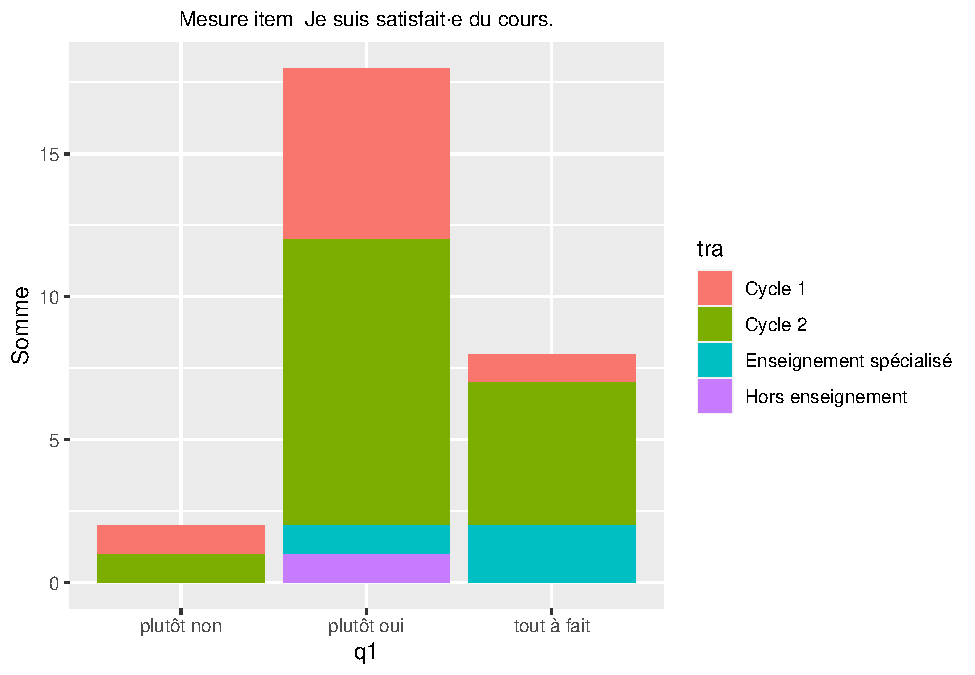
\includegraphics[width=0.5\linewidth]{hepvs2021_33_rapport_files/figure-latex/vis-1} 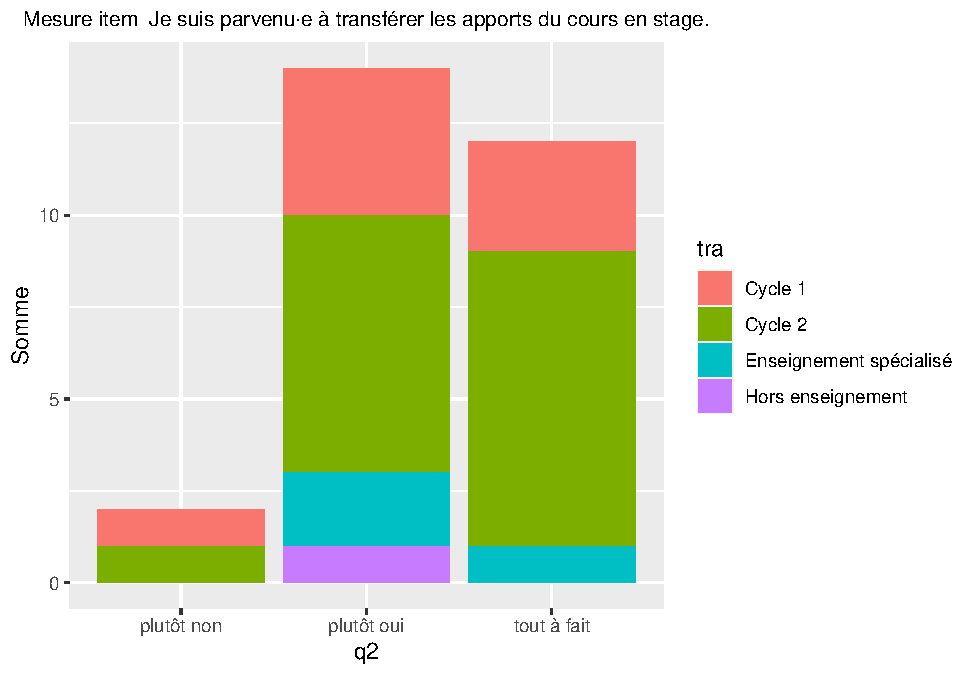
\includegraphics[width=0.5\linewidth]{hepvs2021_33_rapport_files/figure-latex/vis-2} 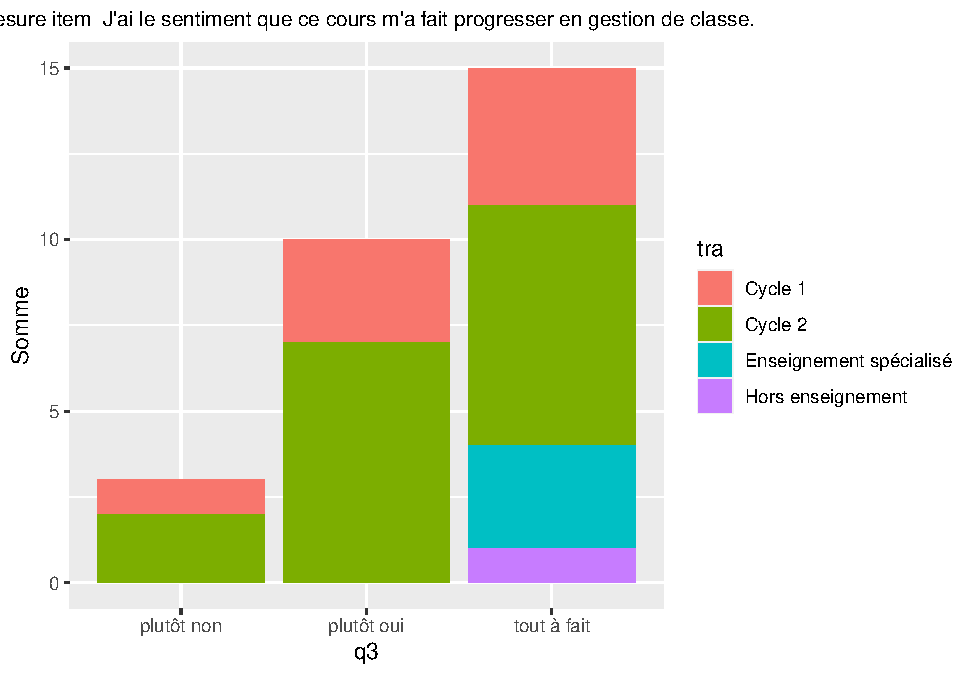
\includegraphics[width=0.5\linewidth]{hepvs2021_33_rapport_files/figure-latex/vis-3} 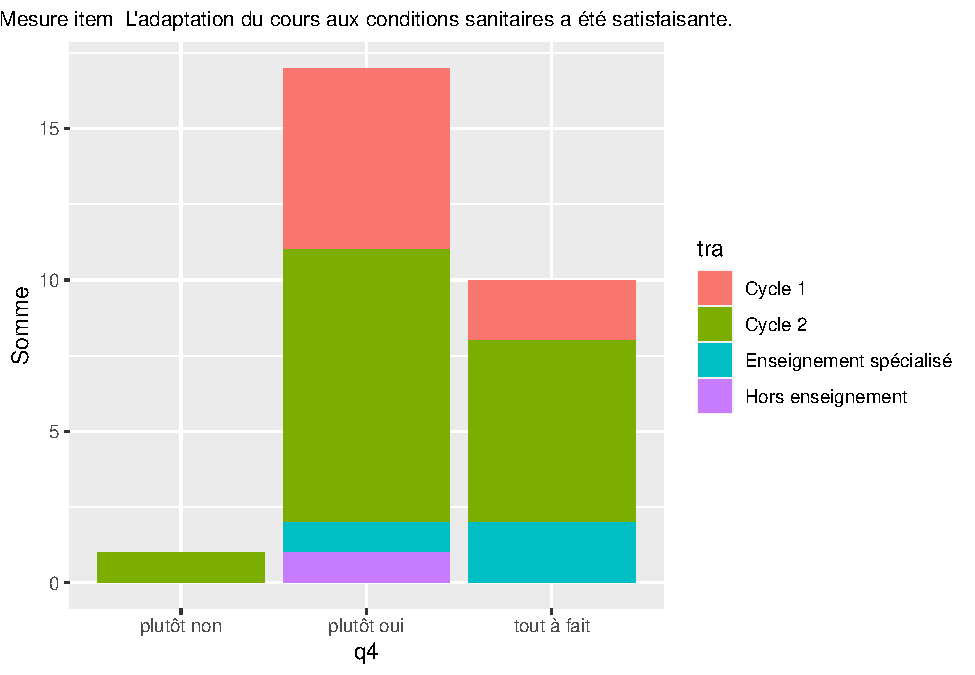
\includegraphics[width=0.5\linewidth]{hepvs2021_33_rapport_files/figure-latex/vis-4}

\hypertarget{retours-qualitatifs}{%
\section{Retours qualitatifs}\label{retours-qualitatifs}}

\hypertarget{forces-du-cours}{%
\subsection{Forces du cours}\label{forces-du-cours}}

Expériences concrètes, partages de choses vécues en stage.
Intéressant, motivant, concret, utile
Nous avons eu des exemples concrets à utiliser en stage. Les concepts m'ont permis d'améliorer ma gestion de classe et de développer les connaissances en climat de classe. La synthèse en mind map est un outil pratique et utile pour l'enseignement
Mettre en pratique ce qui a été enseigné en cours
Hétérogénéité des contenus
La matière est très intéressante et utile.
Demander de faire une carte conceptuelle
Demander de trouver ses propre valeurs et de construire son système de gestion de classe, puis essayer d'appliquer en stage
Les cinq axes et l'exemplification avec des exemples concrets
Les nombreuses ressources
Les apports théoriques et les bienfaits pour le stage.
Un enseignant très disponible et avec une expérience permettant de faire des liens avec le terrain
L'enseignant, très impliqué dans son travail, connaît énormément de choses
Sa disponibilité a été incroyable ! pendant le stage, les permanentes et par mail aussi"
Qualités de l'enseignement
L'élaboration de son propre système de gestion de classe.
Conseils pratiques et enseignant à disposition pour tout problèmes de stage
Différents modèles théoriques de gestion de classe
Prof à l'écoute et présent pour nous aider
L'implication des enseignants, leur disponibilité et leur écoute.
Apports de situations concrètes
Échanges et interactions ponctuelles entre les étudiants et l'enseignant / Enseignant ouvert et bienveillant / Très concret - exemples du terrain très intéressants / Étudiants actifs\ldots{}
Les capsules vidéos qui ne me bloquaient pas dans mon organisation hebdomadaire.
L' apport des expériences professionnelles de M. Massy et sa disponibilité sur Teams pendant le stage.
Ce cours m'a également permis de combler de nombreuses lacunes accumulées lors du premier cours de gestion de classe suivi en allemand à Brigue.
Les sources bibliographiques citées dans les ppt. "
Vidéo explicative très claire
Beaucoup d'apports théoriques
Disponibilité de l'enseignant"
1) Il y a énormément de sources à disposition.
2) Les explications théoriques durant les cours sont claires et exemplifiées.
3) J'ai beaucoup apprécié le fait de pouvoir transférer des éléments du cours en stage (modèle de gestion de classe).
4) Votre bonne humeur, votre motivation et votre bienveillance font parties des forces de ce cours."
Les exemples pour chaque axes de posture
Vous avez exemplifié des concepts avec des exemples de la vie réelle et venant de votre expérience (très riche). Vous nous avez donné beaucoup de pistes concrètes pour nous aider. Les concepts étaient bien expliquées. Vous nous avez donné de votre temps. Selon moi, la principale force de ce cours est Que vous vous intéressiez réellement à comment on allait! Merci.
La clarté de l'enseignante dans sa présentation des concepts
La possibilité de mettre à profit les enseignements du cours dans nos stages
La disponibilité de l'enseignant
La présentation et la mise à disposition de documents théoriques (notamment les modèles de Charles)
Le fil rouge clair et précis du déroulement de la séquence (du thème 3.3)
La possibilité d'évolution à la fois dans notre modèle mais aussi dans notre pensée
L'exposition d'une multitudes d'aspects (axes) de la gestion de classe
Le choix de ce que nous voulions expérimenter en stage ---\textgreater{} identité professionnelle "
Disponibilité
Les séances asynchrones permettaient une grande liberté et c'était super.
Il y avait très peu de travaux de groupe, MERCI ! :)"
Les points forts de ce cours sont les apports théoriques, le lien théorie-pratique par le biais de la carte mentale et la disponibilité de l'enseignant.
La clarté des explications et les discussions très enrichissantes

\hypertarget{faiblesses-du-cours}{%
\subsection{Faiblesses du cours}\label{faiblesses-du-cours}}

Parfois peine à comprendre les concepts, parfois trop rapide
Je trouve que ce cours n'a pas de faiblesses a proprement parlé.
Au début c'était un peu compliqué de comprendre les concepts (modes: conatif,didactique, etc., ainsi que le mode automatique et réflexif)
Peu d'approfondissement des différents troubles
Compliqué à suivre et assimiler la matière des capsules vidéo.
Modalités d'évaluation peu claires, peut-être consacrer plus de temps à expliquer ce qui est attendu dans le dossier et sur la carte conceptuelle
Difficile de comprendre toutes les attentes de l'examen.
Un fil rouge précis
Beaucoup trop théorique, difficile pour moi de trouver de la motivation alors que le concept de gestion de classe m'intéresse vraiment
Pas beaucoup de pistes pratiques pour le cycle 1
J'aurais aimé avoir des pistes plus pratiques, des analyses de cas ou de vidéos comme au semestre 4 m'aurait paru davantage pertinent
Power point vidéo trop long
Pas assez d'échanges entre étudiants
Beaucoup de concepts redondants durant le semestre.
Parfois trop théorique, beaucoup d'apports --\textgreater{} surcharge cognitive
Manque de lien avec la pratique pour des petits degrés. Beaucoup d'idées pour les grands mais difficiles à mettre en place pour des petits
La communication à distance est parfois compliquée.
Théorie trop approfondie
Parfois les apports théoriques étaient trop conséquents et trop rapides, difficile de rester attentifs et concentrés tout du long dans ces moments
Au début du semestre, j'aurais apprécié recevoir le plan du cours détaillé du début à la fin. Surtout de savoir si les distanciels étaient synchrones ou asynchrones afin de m'organiser au mieux.
La distance a permis moins de moments d'échanges.
Par rapport aux cours en présentiels (qui n'ont pas été nombreux malheureusement) j'aurais préféré un peu moins de théorie et plus de pratique, de cas concrets.
Lors des premières séances, il était compliqué de comprendre la structure générale du cours (modalité d'évaluation, modalité de la tâche associée en stage, etc.) Il me paraissait compliqué de lier le cours, l'évaluation et le stage.
Cours quasiment que frontal et transmission
Manque de pratique et d'élément concrets
La seule chose qui m'a été parfois difficile était la mise en page de certaines slides du ppt. Mais comme vous l'expliquiez après, ça ne posait plus problème.
Les aspects théoriques assez complexes et difficiles à cerner. De plus ils étaient abondants et pas assez reliés à la pratique (dans la présentation du cours)
Le manque d'exemples concrets
Le manque d'échanges avec les partenaires sur les aspects de la gestion de classe
Le fait d'imposer une carte conceptuelle pour le modèle de gestion de class
J'ai l'impression qu'il y avait beaucoup de pistes pour le cycle 2 ou encore pour des adolescents, et moins de pistes pour la gestion de classe au cycle 1.
Il y a beaucoup de théorie mais les exemples concrets de Monsieur Massy ont permis de bien l'intégrer.
Le cour est parfois difficile en terme de nouveau concept à intégrer et le distanciel rend l'intégration plus lente.
Plus de référence au cycle 1

\hypertarget{pistes-damuxe9lioration-proposuxe9es}{%
\subsection{Pistes d'amélioration proposées}\label{pistes-damuxe9lioration-proposuxe9es}}

Donner des exemples concrets
Mieux expliciter les modalités d'évaluation et la création de la carte. Aller moins vite lors de la présentation des concepts. Peut-être aborder moins de théorie mais en l'expliquant davantage et en entrant plus dans les détails et donner des exemples.
Langage de cours peut-être moins complexe
Construction d'un document physique regroupant uniquement des pistes d'action nous permettant d'être utile en stage
Plus de cours Teams où il est possible de poser des questions.
Présenter au début du module, comme pour le Gestion et Climat de classe I, les modalités d'évaluation et ce qui est attendu dans le dossier d'évaluation
Des explications en présentiel. Le mercredi après-midi nous devions travailler pour le stage \ldots{}
Une présentation avec un fil rouge plus précis en début de semestre
Utiliser des vidéos pour analyser le comportement d'un enseignant peut-être
Démontrer des pratiques, faire des jeux de rôles pour que l'on se rende vraiment compte de ce que l'on demande aux élèves
L'enseignant avait l'air d'avoir beaucoup de vécu --\textgreater{} nous expliquer des situations, comment il a fait, des pistes pratiques pour nous aider
Moins de théorie
Faire des activités en sous groupe pour pouvoir davantage échanger entre nous
Parler plus de situations vécues en stage afin de trouver des pistes
Plus travailler les différentes théories ex: travail de groupe pour illustrer par ex le modèle skinérien
Faire plus de lien entre la pratique et la théorie
Varier les supports de cours
Plus de cas concrets
Répartir les longs moments théoriques, les couper avec des moments plus actifs
Etablir un plan détaillé du cours pour les étudiants.
Proposer des situations (ou récolter nos situations problématiques en début de semestre), réfléchir à des manières d'intervenir, confronter nos idées\ldots{}
Je propose de présenter différemment l'activité liée au stage.\\
Continuer de partir des situations des élèves ?
Des cours qui sont plus orientés vers des situations problèmes (scénette,.. )
Je n'ai pas de piste d'amélioration à proposer, je pense que c'était l'un des meilleurs cours que j'ai durant mes 3 ans de HEP! J'aurai apprécié suivre ce cours en présentiel mais pas le choix\ldots{} Merci pour tous ces apports, j'ai noté une nette amélioration dans ma gestion de classe.
Plus d'exemples qui permettraient de mieux cerner les aspects théoriques
Plus d'échanges avec ses collègues pour s'approprier les concepts
Laisser le choix de présentation du modèle de gestion de classe
Apporter plus de contenus concernant la gestion de classe dans les petits degrés.
Il était GENIAL
Pour pouvoir comprendre certains concepts, j'ajouterai des versions écrites des cours avec définition des théories, les capsules n'étant pas le plus pratique pour revoir les concepts.
Un bilan intermédiaire de nos modèle de gestion de classe après le retour de stage. Une sorte de présentation à la classe de chaque élève.

\hypertarget{synthuxe8se-de-luxe9quipe-de-formation}{%
\section{Synthèse de l'équipe de formation}\label{synthuxe8se-de-luxe9quipe-de-formation}}

Comment on interprète.

Ce qu'on vise.

\end{document}
